\section{VS Code Configuration for WSL}

You are free to use whatever text editor that you like.
If you use VS Code, however, you can apply the following configuration to get code completion and code navigation to work.
This configuration is tailored towards Zephyr development inside a WSL distro.

\begin{itemize}
  \item Install the \href{https://marketplace.visualstudio.com/items?itemName=ms-vscode-remote.remote-wsl}{WSL extension}
  \item Connect to WSL distro using the 
\includegraphics[height=.8em]{vscode_connect_button} button on the bottom left (\emph{Connect to WSL using Distro...})
  \item Clangd searches for a compilation database file (\mono{compile_commands.json}) in the parent directories of source files and also in subdirectories named \mono{build} (see \href{https://clangd.llvm.org/installation#project-setup}{documentation}).
    If you build your project in \mono{/tmp/build}, clangd will not find the database file.
    Run the following command to create a link to the compilation database file such that clangd can find it (adapt the paths as needed).

\begin{monobox}
@\cmdinwsl{}@ ln -s `
  /tmp/build/compile_commands.json `
  /mnt/c/path/to/zephyr/project/
\end{monobox}
  \item Create a file named \mono{.clangd} in the same location where you created the link to the compilation database file.
    Copy the following to this file (make sure that the indentation is the same as here).

\begin{monobox}
CompileFlags:
  Remove:
    - '-fno-printf-return-value'
    - '-fno-reorder-functions'
    - '-mfp16-format=ieee'
\end{monobox}
  \item Install the \href{https://marketplace.visualstudio.com/items?itemName=llvm-vs-code-extensions.vscode-clangd}{LLVM clangd} extension.
    Make sure to install the extension while you are connected to the WSL.

    When you see the following pop-up, click on \emph{Install}.
    \begin{center}
      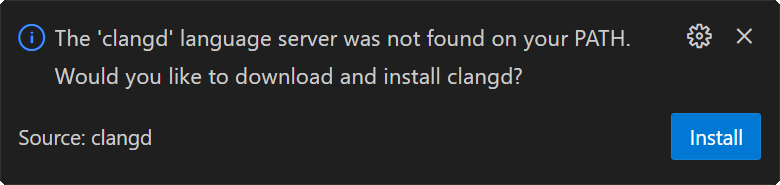
\includegraphics[width=.7\textwidth]{clangd_quick_time_event.png}
    \end{center}
  \item Open the project folder via \emph{File} $\rightarrow$ \emph{Open Folder...} $\rightarrow$ \mono{/mnt/c/...}
\end{itemize}
